% -*- Mode:TeX -*-
\documentclass[twocolumn]{cinc}
\usepackage{graphicx}
\begin{document}
\bibliographystyle{cinc}

\title{Spectral Analysis of Heart Rate Without Resampling}

\author {
GB Moody\\
\ \\
Harvard-M.I.T. Division of Health Sciences and Technology, Cambridge, MA, USA}

\maketitle

\begin{abstract}
Standard methods of estimating the power spectral density (PSD)
of irregularly sampled signals such as instantaneous heart rate (HR)
require resampling at uniform intervals and replacement of unusable
samples.  The Lomb periodogram is a means of obtaining PSD estimates
directly from irregularly sampled time series, avoiding these
requirements.  This paper compares Fourier, autoregressive, and Lomb
PSD estimates from synthetic, real, and noise-corrupted real heart
rate time series, and examines systematic differences among these
estimates.  An algorithm is presented for obtaining a heart rate time
series suitable for Lomb PSD estimation from an RR interval time
series with included ectopic beats and erroneous measurements.  The
paper concludes with a brief survey of other applications of the
technique, such as estimation of respiratory frequency from a time
series of beat-by-beat measurements of the mean electrical axis.
\end{abstract}

\section{Introduction}

Power spectral density estimation is a commonly-used analytic
technique for describing periodicities in time series.  Most
non-trivial analyses of heart rate variability (HRV) depend on PSD
estimation.  The instantaneous heart rate time series used as the
bases of these analyses are sampled at intrinsically irregular
intervals (if the RR intervals were uniform, there would be no HRV to
analyze).  Standard methods for PSD estimation, including Fourier
transform (FT) and autoregressive (AR) methods, operate on time series
with uniform intervals between samples.  To apply FT or AR techniques
to heart rate time series therefore requires that the series be {\em
resampled} at uniform intervals\cite{RD-84,RB-86,GM-92}.  The
resampling process alters the frequency content of even a noise-free
time series by nonlinear low-pass filtering (Figure\ref{fig:timeseries}).

If the time series contains inappropriate or missing samples (as, for
example, in heart rate time series with ectopic beats or noise), PSD
estimates can be severely affected, since impulse noise in the time
domain is transformed to broad-band ``clutter'' in the frequency
domain.  In such cases, resampling is further complicated by the need
to infer probable values as replacements\cite{PA-88}, with the
likelihood of further alteration of frequency content\cite{CB-91}.
For these reasons, some investigators analyze only segments free of
ectopy and noise\cite{RK-87}; this approach runs the risk of
introducing selection bias in HRV analysis, however, since both ectopy
and noise are correlated with HRV-related factors such as physical
activity.

Methods for PSD estimation based directly on irregularly sampled time
series have been used, though not in HRV analysis, since at least
1976\cite{NL-76,RJ-81}.  Methods such as the Lomb periodogram
entirely avoid the problems associated with resampling and sample
replacement.  The high computational burden of these methods has been
a major obstacle to their general use\cite{RB-92} until recently.  In
1989, Press and Rybicki published a fast algorithm for obtaining an
arbitrarily accurate approximation to the Lomb
periodogram\cite{WP-89,NR-92}.  The remainder of this paper
illustrates how the Lomb periodogram, obtained using the Press-Rybicki
algorithm, may be applied to analysis of HRV and related signals.

\section{Examples}

Several HR time series are presented below, together with the
corresponding Lomb, FT, and AR spectra.  In each case, an irregularly
sampled instantaneous heart rate (IHR) signal was obtained from an RR
interval time series using the algorithm given in the appendix, and
this signal was used as input to the Press-Rybicki algorithm to obtain
the Lomb periodogram.  A regularly sampled instantaneous heart rate
signal\cite{GM-92} was obtained from the same RR series; this signal
(five minutes in length in each case, and sampled at 2 Hz) was
zero-meaned, detrended, zero-padded to a length of 1024 samples, and
Welch windowed, and the result was used as input to standard fast
Fourier transform (FT) and autoregressive model (AR) algorithms for
PSD estimation\cite{NR-92}.  In the examples shown here, the AR models
are of order 24.  The Lomb and AR spectra can be evaluated for any
desired frequencies; for purposes of comparison, all spectra were
evaluated at the discrete frequencies defined for the Fourier spectra.

To demonstrate the essential similarity of FT, AR, and Lomb PSD estimates,
synthesized HR time series are shown in Figures~\ref{fig:timeseries} and
\ref{fig:spectra}.

\begin{figure}
\centerline{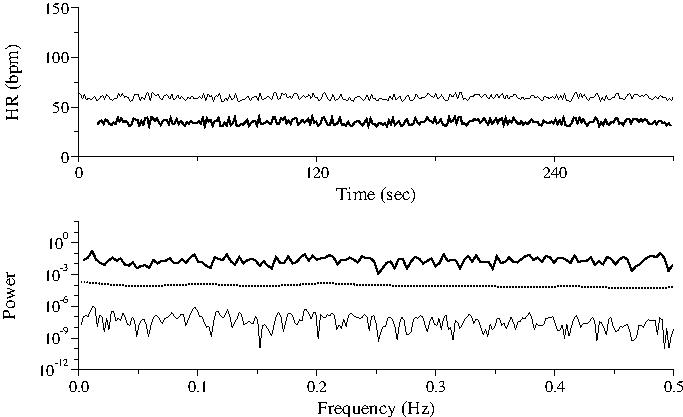
\includegraphics[width=8cm] {figures/fig1}}
%\vspace{1cm}
  \caption{\label{fig:timeseries} Synthesized HR time series and corresponding spectra (see text).
    In Figures 1--5, the upper trace is the resampled HR series used to
    derive the FT and AR spectra; below it is the IHR series (offset by 25
    bpm for clarity) used to derive the Lomb spectrum.  The lower panel
    shows, from top to bottom: the Lomb spectrum (heavy line); the AR
    spectrum (dotted line); and the FT spectrum (thin line).  For clarity,
    the AR and FT spectra are offset by $10^{3}$ and $10^{6}$ units
    respectively.}
\end{figure}

These five-minute sequences were generated using a recurrence of the form
\begin{equation}
RR_{i} = a_{0} + a_{1} \sin ( {\omega_{1} t_{i} + \phi_{1}} ) +
 a_{2} \sin ( {\omega_{2} t_{i} + \phi_{2}} ) + a_{3} z
\end{equation}
\begin{equation}
t_{i+1} = t_{i} + RR_{i}
\end{equation}
where $RR_{i}$ is the RR interval beginning at $t_{i}$, $z$ is a random
variable evenly distributed between -1 and 1, and the remaining parameters
are arbitrary constants.  For the simulation shown in Figure 1, both
$a_{1}$ and $a_{2}$ are 0, so that the sequence contains randomly-varying
intervals with a mean of $a_0$ (1 second in the simulations shown here).
The Lomb periodogram of this sequence is consistent with white noise,
whereas the FT and AR spectra show the high-frequency (HF) attenuation
expected as a result of the resampling process.  In
Figure~\ref{fig:spectra}, $a_{1}$ and $a_{2}$ are equal and larger than
$a_{3}$; $\omega_{1}$ and $\omega_{2}$ are chosen to modulate the RR
intervals at frequencies of 0.05 and 0.41 Hz, to simulate
sympathetically-mediated low frequency HR oscillations and
parasympathetically-mediated respiratory sinus arrhythmia.  The three
spectra are quite similar, apart from the HF attenuation in the FT and AR
spectra, and the lack of detail/clutter in the AR spectrum.

\begin{figure}
    \centerline{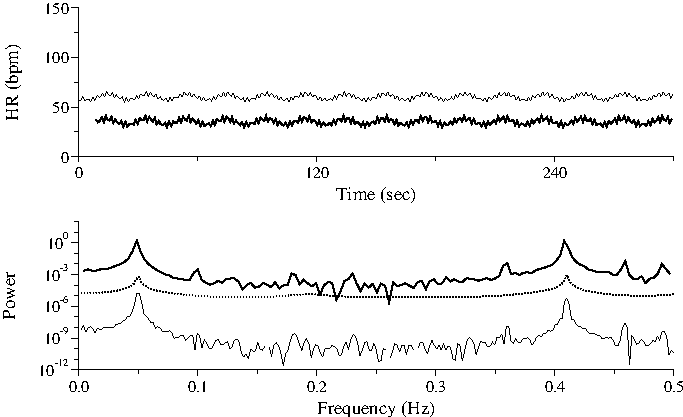
\includegraphics [width=8cm] {figures/fig2}}
    % \vspace{1cm}
    \caption{\label{fig:spectra} Synthesized HR time series and corresponding
      spectra (see text).}
\end{figure}

The sequence in Figure~\ref{fig:apnea} was obtained by automated analysis
of an ECG signal acquired from a subject with sleep apnea syndrome; the low
frequency modulation of heart rate with a period of roughly 45 seconds
matches the frequency of the subject's obstructive apneas.  Although the
spectral peak near 0.025 Hz is most obvious in the AR spectrum, it is also
clearly visible in both the Lomb and the FT spectra, which also reveal the
harmonically related peak near 0.05 Hz.

The sequence in Figure~\ref{fig:noise} was obtained by automated analysis
of the same signal used in Figure~\ref{fig:apnea}, after addition of
electrode motion artifact scaled to obtain a signal-to-noise ratio of 12
dB.  Roughly 30 QRS detector errors resulting from the added noise are
readily discernible in the time series.  Although much of the sequence is
rejected by the algorithm that prepares input for the Lomb periodogram, the
peak near 0.025 Hz is still prominent, and the first harmonic also remains
visible.  The 0.025 Hz peak is visible but not significant among the
clutter in the FT spectrum, and the AR spectrum has no significant
features.

By rejecting the outliers and using a
predictive interpolator to obtain replacement samples, as shown in
Figure 5, the 0.025 Hz peak emerges as a broad feature in the AR
spectrum, but the FT spectrum shows a broad, spurious peak at about
0.015 Hz.

Other irregularly-sampled time series frequently appear in HRV-related
studies.  Among those amenable to Lomb PSD analysis are respiration
intervals and tidal volumes, gait, and beat-by-beat systolic blood
pressure measurements.  As a final example, Figure~\ref{fig:Lomb} shows a time
series of beat-by-beat measurements of the mean cardiac electrical
axis, which fluctuates in response to respiration\cite{GM-85};  the
Lomb spectrum clearly reveals the respiratory frequency.

\begin{figure}[t]
    \centerline{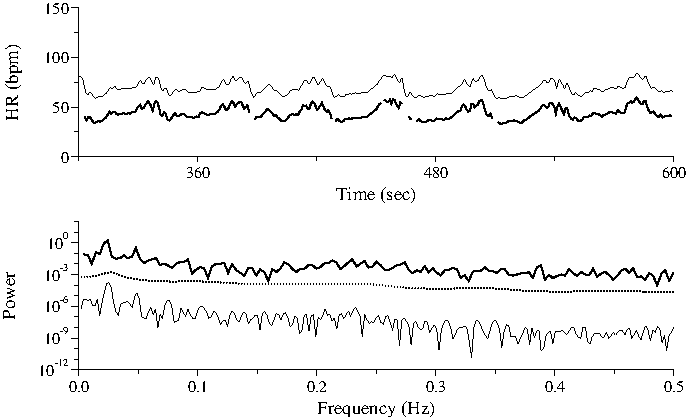
\includegraphics[width=8cm] {figures/fig3}}
    % \vspace{1cm}
    \caption{\label{fig:apnea} HR time series and spectra during periodic
      obstructive apneas.}
\end{figure}

\begin{figure}[ht!]
    \centerline{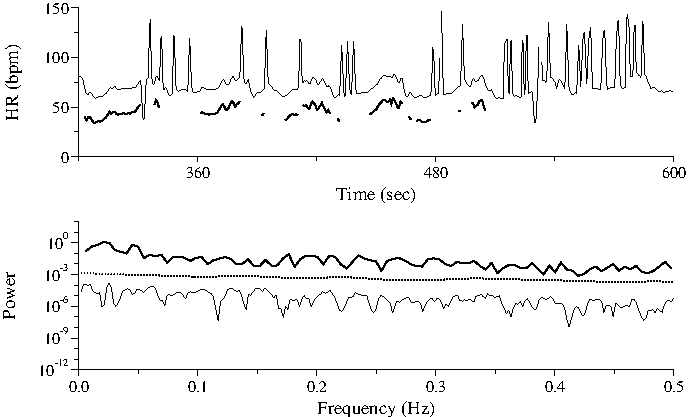
\includegraphics[width=8cm] {figures/fig4}}
    \caption{\label{fig:noise} HR time series from Figure 3, corrupted by
      added noise, with corresponding spectra.}
\end{figure}

\begin{figure}[ht!]
    \centerline{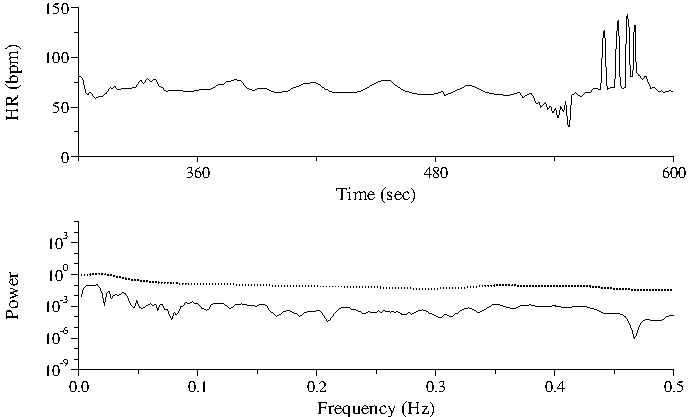
\includegraphics[width=8cm] {figures/fig5}}
    \caption{\label{fig:corrected} HR time series from Figure 4, corrected
      using a predictive interpolator, with corresponding AR and FT
      spectra.}
\end{figure}

\begin{figure}
    \centerline{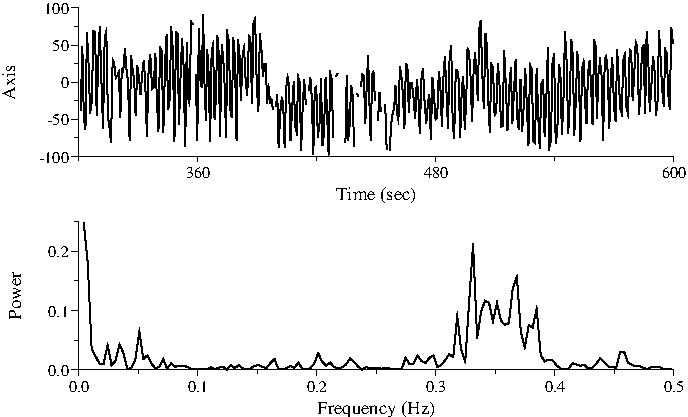
\includegraphics[width=8cm] {figures/fig6}}
    \caption{\label{fig:Lomb} Electrical axis time series (above), with Lomb
      spectrum (below).}
\end{figure}

\section{Conclusions}

Lomb and FT spectra are derived using $O(N \log N)$ algorithms,
and AR spectra are derived using an algorithm that is only slightly
slower for reasonable choices of model order.  The essential
similarity of the Lomb, FT, and AR spectra given ideal inputs,
considered in light of their similar computational demands, suggests
that there may be little reason to choose one over any other.
When considering the less-than-ideal inputs endemic to HRV studies,
however, only the Lomb method produces robust PSD estimates in the
presence of noise and ectopy.  The Lomb method avoids all of the
complications and pitfalls of resampling and replacement of outliers,
and introduces no drawbacks of its own; in consequence, it is the
method of choice for PSD estimation of heart rate.

\section*{Acknowledgements}

This work was supported in part by grants from the National Institute
on Drug Abuse (P01-DA06316); the National Heart, Lung, and Blood
Institute (R01-HL-42172); the National Aeronautics and Space
Administration (NAG9-572); and the G. Harold and Leila Y. Mathers
Charitable Foundation.

\bibliography{bib/psd}

\vspace*{4mm}
\appendix{}

The C program below generates an instantaneous heart rate (HR) signal
suitable for Lomb PSD estimation.  Its input should be a two-column
list of beat arrival times (in seconds) and beat type codes (1 for
normal beats, any other value for other types of beats).  The output
contains a subset of the beat arrival times, with a sample of the HR
signal (in units of beats per minute) following each time.  The {\tt
scanf} and {\tt printf} statements may be replaced if different input
or output formats are required.
\balance

Note that this algorithm aggressively rejects intervals likely to be
outliers (whether due to ectopic beats, falsely detected beats,
missed beats, or simply mismeasured beat arrival times).  When used to
derive a Lomb PSD estimate, this strategy works well, and permits
robust derivation of spectra even from highly corrupted time series.
When deriving FT or AR spectra, less stringent criteria must be used,
since the cost of deleting samples is high (either they must be
replaced, or the entire time series must be discarded).

{\small
\begin{verbatim}
#include <stdio.h>
#include <math.h>
#define NORMAL 1
#define OTHER  2
#define TOL   10    /* tolerance (bpm) */

main()
{
    double ihr, ihrp, mhr = 70., t, tp;
    int b, bp = OTHER;

    while (scanf("%lf%d", &t, &b) == 2) {
        if (b == NORMAL) {
            ihr = 60./(t - tp);
            mhr += (ihr - mhr)/10.;
            if (bp == NORMAL &&
                fabs(ihr - ihrp) < TOL &&
                fabs(ihr - mhr) < TOL)
                printf("%g %g\n", tp, ihr);
            bp = NORMAL;
            tp = t;
            ihrp = ihr;
        }
        else
            bp = OTHER;
    }
}
\end{verbatim}
}

\vspace*{-.6cm} %adjustment to make the columns even
\begin{correspondence}
George B. Moody\\
MIT Room E25-505A, Cambridge, MA 02139 USA.\\
george@mit.edu
\end{correspondence}
\end{document}

Author's note: This paper originally appeared in Computers in Cardiology 1993,
pp 715-718.  The figures have been regenerated from the original data, the
address for correspondence has been updated, the LaTeX formatting commands have
been changed to make use of the cinc macros, and this paragraph (which does not
appear in the printed version, since it follows the end-of-document statement
above) has been added.  No other changes have been made.
